%!TEX root = ./workbook-2011.tex

\section{Writing Functions in R}

So far we've been mostly using R's built in functions. However the power of a
true programming language is the ability to write your own functions.

The general form of an R function is as follows:

\begin{R}
funcname <- function(arg1, arg2) {
 # one or more expressions
 # last expression is the object returned
 # or you can explicitly return an object
}
\end{R}
To make this concrete, here's an example where we define a function in
the interpreter and then put it to use:
%
\begin{R}
> myfunc <- function(x,y){
+ # don't type the '+' symbols, these show continuation lines
+   x^2 + y^2
+ }

> a <- 1:5
> b <- 6:10
> a
[1] 1 2 3 4 5
> b
[1]  6  7  8  9 10
> myfunc(a,b)
[1]  37  53  73  97 125
> myfunc
function(x,y){
  x^2 + y^2
}
\end{R}
%
If you type a function name without parentheses R shows you the
function's definition. This works for built-in functions as well
(thought sometimes these functions are defined in C code in which case R
will tell you that the function is a `.Primitive').

\subsection{Putting R functions in Scripts}

When you define a function at the interactive prompt and then close the
interpreter your function definition will be lost. The simple way around
this is to define your R functions in a script that you can than access
at any time.

Choose \lstinline!File > New Script! (or \lstinline!File > New Document! in OS
X) in the R GUI . This
will bring up a blank editor window. Enter your function into the editor
and save the source file in your R working directory with a name like
\lstinline!vecgeom.R!.

\begin{R}
# functions defined in vecgeom.R

veclength <- function(x) {
  # Given a numeric vector, returns length of that vector
  sqrt(drop(x %*% x))
}

unitvector <- function(x) {
  # Return a unit vector in the same direction as x
  x/veclength(x)
}

vec.cos <- function(x,y) {
  # Calculate the cos of the angle between vectors x and y
  len.x <- veclength(x)
  len.y <- veclength(y)
  return( (x %*% y)/(len.x * len.y) )
}

\end{R}
There are two functions defined above, one of which calls the other.
Both take single vector arguments. At this point there is no error
checking to insure that the argument is reasonable but R's built in
error handling will do just fine for now.

Once your functions are in a script file you can make them accesible by
using the \lstinline!source()! function (See also the
\lstinline!File > Source R code...! menu item in the R GUI):
%
\begin{R}
> source("vecgeom.R")
> x <- c(1,0.4)
> veclength(x)
[1] 1.077033
> ux <- unitvector(x)
> ux
[1] 0.9284767 0.3713907
> veclength(ux)
[1] 1
\end{R}

Let's also add the following function to |vecgeom.R| to aid in visualizaing 2D vectors:
%
\begin{R}
draw.vectors <- function(a, b, colors=c('red', 'blue'), clear.plot=TRUE){

    # figure out the limits such that the origin and the vector
    # end points are all included in the plot
    xhi <- max(0, a[1], b[1])
    xlo <- min(0, a[1], b[1])
    yhi <- max(0, a[2], b[2])
    ylo <- min(0, a[2], b[2])

    xlims <- c(xlo, xhi)*1.10 # give a little breathing space around vectors
    ylims <- c(ylo, yhi)*1.10

    if (clear.plot){
        plot(xlims, ylims, type='n', asp=1, xlab="x-coord", ylab="y-coord")
    }
    arrows(0, 0, a[1], a[2], length=0.1, col=colors[1])
    arrows(0, 0, b[1], b[2], length=0.1, col=colors[2])
}
\end{R}
%
You can use this new function as follows:
\begin{R}
# you need to source the file everytime you change it
> source("/Users/pmagwene/Downloads/vecgeom.R")
> x <- c(1,0.4)
> y <- c(0.2, 0.8)
> draw.vectors(x,y)  # draw the original vectors
\end{R}
%
The resulting figure should resemble the one below.
%
\begin{figure}[htbp]
\centering
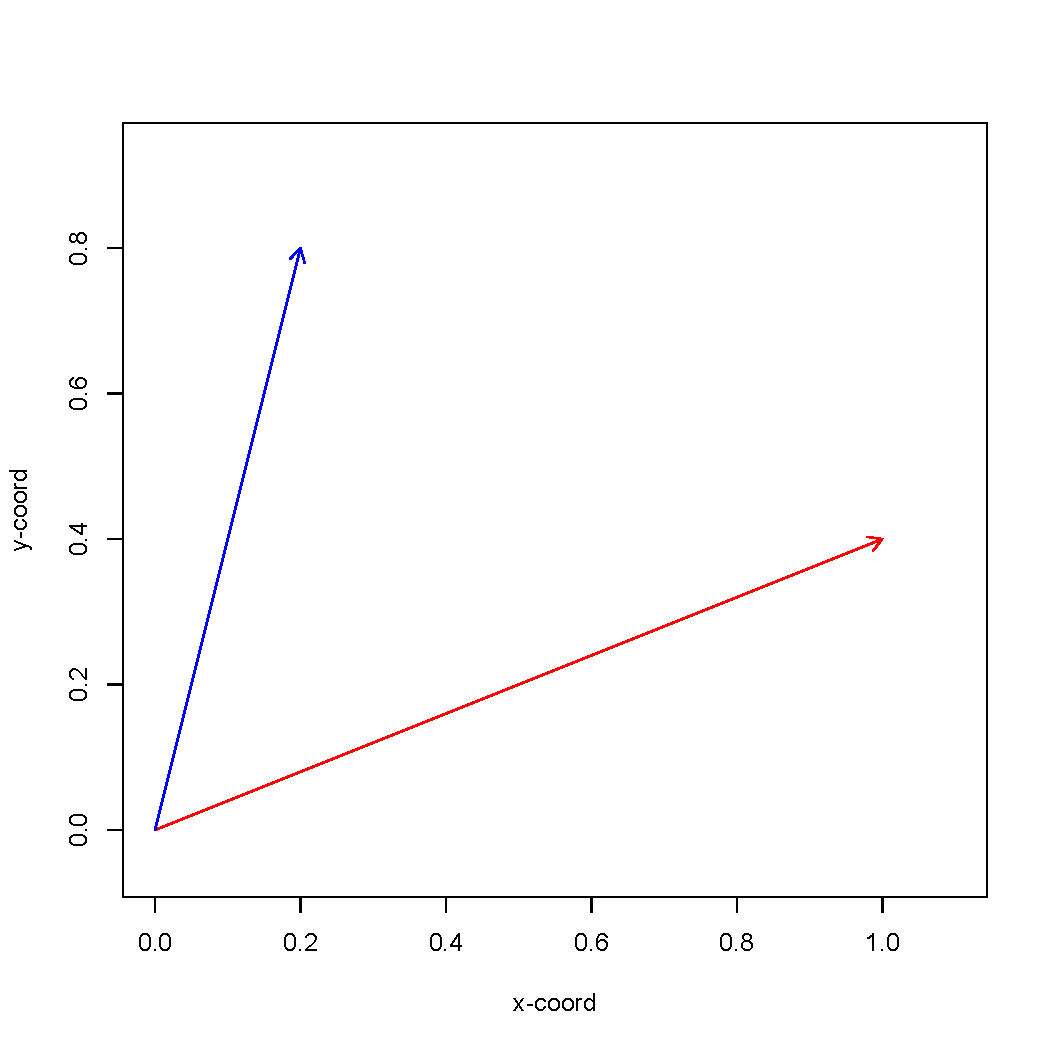
\includegraphics[width=0.33\columnwidth]{./figures/hands-on2/vecfig2.pdf}
\caption{Another vector figure.}
\end{figure}

Notice that we included a |clear.plot| argument in our |draw.vectors| function. I included this so we could add additional vectors to our plot, without overwriting the old vectors, as demonstrated below:
\begin{R}
# draw the unit vectors that point in the same directors as the original vectors
> ux <- unitvector(x)
> uy <- unitvector(y)
> draw.vectors(ux, uy, colors=c('black', 'green'), clear.plot=F)
\end{R}

\begin{assignment}
Write a function in R that takes two vectors, $\vec{x}$ and $\vec{y}$, and returns a list containing the projection of $\vec{y}$ on $\vec{x}$ and the component of $\vec{y}$ in $\vec{x}$:

\lstDeleteShortInline|

\[P_{\vec{x}}(\vec{y}) = \left(\frac{\vec{x} \cdot \vec{y}}{|\vec{x}|}\right) \frac{\vec{x}}{|\vec{x}|}\]
and
\[C_{\vec{x}}(\vec{y}) = \frac{\vec{x} \cdot \vec{y}}{|\vec{x}|}\]

\lstMakeShortInline|

\end{assignment}

